\documentclass[11pt]{ctexart}
\usepackage[a4paper,margin=1in]{geometry}
\usepackage{amsmath,amssymb}
\usepackage{booktabs}
\usepackage{longtable}
\usepackage{graphicx}
\usepackage{float}
\usepackage{hyperref}
\hypersetup{colorlinks=true,linkcolor=blue,urlcolor=blue}

\title{固定 Tucker 秩 \texorpdfstring{$[2,5,2]$}{[2,5,2]} 的 \texttt{tsrProj} 统计推断说明}
\author{}
\date{\today}

\begin{document}
\maketitle

\section{任务与背景}
本文档记录在 ROI10 EEG 张量回归中，固定 Tucker 秩为 $[2,5,2]$ 后，利用 \texttt{tsrProj.m} 进行线性泛函推断的完整操作步骤与结果。这里的分析可视为在主分析之外的一次固定秩敏感性分析。

协变量张量为 $10\times 8\times 2$，分别对应 ROI、频段和状态（EC/EO）；响应变量为年龄。张量回归中使用的协变量构造为
\[
X_i = \bigl(\log_{10}(\mathrm{EC}_i), \log_{10}(\mathrm{EO}_i)\bigr),
\]
其中对原始 band power 先做正值下界截断，再取 $\log_{10}$。本次分析固定秩为 $[2,5,2]$，不重新做 rank selection。

\section{数据与推断对象}
数据文件为 \texttt{hbn\_bandpower\_8band\_roi10.mat}，其中每个受试者都有：
\begin{itemize}
\item $10$ 个 ROI group；
\item $8$ 个 canonical frequency bands；
\item $2$ 个 resting-state conditions（EC 与 EO）；
\item 年龄变量 \texttt{age}。
\end{itemize}

本次推断保留与既往 \texttt{tsrProj} 分析相同的 $205$ 个预先设定 loading，并统一进行 Frobenius norm 归一化：
\begin{itemize}
\item $160$ 个 single-element loadings；
\item $10$ 个 ROI-slice loadings；
\item $8$ 个 band-slice loadings；
\item $2$ 个 condition-slice loadings；
\item $1$ 个 full-tensor loading；
\item $1+8+3$ 个 shared loadings；
\item $1+8+3$ 个 contrast loadings。
\end{itemize}

其中 shared 和 contrast 在第 3 个 mode 上分别取
\[
\frac{(1,1)}{\sqrt{2}},\qquad \frac{(1,-1)}{\sqrt{2}}.
\]

\section{\texttt{tsrProj} 的计算步骤}
对每一个 loading tensor $T$，重复以下步骤：
\begin{enumerate}
\item 读取固定秩 $[2,5,2]$。
\item 对 loading 做 Frobenius norm 归一化，使得 $\|T\|_F=1$。
\item 在 \texttt{tsrProj.m} 中对全样本做随机二折 sample splitting。
\item 对每个 half-sample，使用 training half 的均值对 $X$ 与 $y$ 做 fold-specific centering。
\item 在 centered training half 上调用 \texttt{fit\_tucker\_tensor\_regression.m}，以 Tucker 秩 $[2,5,2]$ 拟合初始低秩估计。
\item 基于 centered second moments 构造 $S_1,S_2,S_3$ 和平均 Frobenius 二阶矩。
\item 利用 \texttt{P\_sigma.m} 与 \texttt{phi\_sigma.m} 计算投影修正项和 projection direction $\Phi$。
\item 交叉利用另一半样本计算残差均值修正，得到 cross-fitted 线性泛函估计 $\hat\delta$。
\item 将两折结果平均，得到最终的 \texttt{thetahat}。
\item 用 cross-fitted residuals 估计 $\sigma^2$，进而得到标准差估计 \texttt{sdest}。
\item 构造 Wald 型置信区间
\[
\hat\delta \pm 1.9599639845 \cdot \frac{\widehat{\mathrm{sd}}}{\sqrt{N}}.
\]
\end{enumerate}

本次运行中，\texttt{run\_roi10\_tsrproj\_loading\_ci\_analysis.m} 使用了更规范的 fold-specific centering 版 \texttt{tsrProj.m}，因此 projection direction $\Phi$、$\sigma^2$ 估计以及最终方差二次型均基于 centered $X^c$ 与 $y^c$。

\section{实现细节}
\subsection{为什么采用分块运行}
直接在一个 MATLAB 进程中顺序计算全部 $205$ 个 loadings 时，会出现 heap corruption，导致长作业在后段中断。为避免整批结果丢失，本次对
\texttt{run\_roi10\_tsrproj\_loading\_ci\_analysis.m}
做了两点最小修改：
\begin{itemize}
\item 增加 \texttt{loading\_start} 与 \texttt{loading\_end} 参数，用于只计算某一段 loadings；
\item 增加 \texttt{make\_plots} 参数，在分块运行时跳过不完整数据上的画图步骤。
\end{itemize}

随后将全部 $205$ 个 loadings 拆成若干小块运行：
\[
1{:}10,\ 11{:}20,\ \ldots,\ 191{:}200,\ 201{:}205.
\]
每个 chunk 都写出自己的
\texttt{tsrproj\_loading\_ci\_all\_results.csv}，
最后再合并成完整结果文件。

\subsection{数值设置}
本次固定设置包括：
\begin{itemize}
\item 推断秩：$[2,5,2]$；
\item split seed：\texttt{20260322}；
\item Tensor Toolbox：\texttt{H:\textbackslash U盘备份\textbackslash 各种方法\textbackslash tensor\_toolbox-v3.6}；
\item 所有 loadings 均使用 Frobenius norm 归一化。
\end{itemize}

\section{结果文件}
完整结果保存在：
\begin{itemize}
\item \texttt{tsrproj\_loading\_ci\_all\_results.csv}
\item \texttt{tsrproj\_loading\_ci\_summary\_counts.csv}
\item \texttt{tsrproj\_loading\_ci\_structured\_results.csv}
\item \texttt{tsrproj\_loading\_ci\_structured\_results\_significant.csv}
\item \texttt{tsrproj\_rank252\_structured\_loadings.png}
\item \texttt{tsrproj\_rank252\_shared\_contrast\_loadings.png}
\end{itemize}

\section{显著性汇总}
表~\ref{tab:count} 汇总了各类 loading 中 95\% 置信区间不包含 $0$ 的个数。

\begin{table}[H]
\centering
\caption{固定秩 $[2,5,2]$ 下各类 loading 的显著性计数}
\label{tab:count}
\begin{tabular}{lcc}
\toprule
Loading type & Count & CI excludes 0 \\
\midrule
single-element & 160 & 140 \\
ROI-slice & 10 & 1 \\
band-slice & 8 & 5 \\
condition-slice & 2 & 0 \\
full-tensor & 1 & 0 \\
shared-global & 1 & 0 \\
shared-band & 8 & 5 \\
shared-ROI-group & 3 & 1 \\
contrast-global & 1 & 0 \\
contrast-band & 8 & 6 \\
contrast-ROI-group & 3 & 0 \\
\bottomrule
\end{tabular}
\end{table}

从表~\ref{tab:count} 可以看出，固定秩 $[2,5,2]$ 下最强的信号仍然集中在 single-element 层面；而在结构化 summaries 中，band-related directions 比 global 或 condition-level directions 更稳定。

\section{结构化推断结果}
表~\ref{tab:structured} 给出本次分析中置信区间不包含 $0$ 的主要 structured loadings。

\begin{longtable}{llrr}
\caption{固定秩 $[2,5,2]$ 下显著的 structured loadings}\\
\toprule
Type & Loading & $\hat\delta$ & 95\% CI \\
\midrule
\endfirsthead
\toprule
Type & Loading & $\hat\delta$ & 95\% CI \\
\midrule
\endhead
ROI-slice & central\_left & $-0.611$ & $[-1.027,\,-0.194]$ \\
band-slice & theta & $-1.671$ & $[-2.307,\,-1.034]$ \\
band-slice & alpha2 & $1.142$ & $[0.775,\,1.510]$ \\
band-slice & beta1 & $0.989$ & $[0.241,\,1.737]$ \\
band-slice & gamma1 & $-1.692$ & $[-2.861,\,-0.524]$ \\
band-slice & gamma2 & $0.988$ & $[0.176,\,1.801]$ \\
shared-band & theta & $-1.671$ & $[-2.307,\,-1.034]$ \\
shared-band & alpha2 & $1.142$ & $[0.775,\,1.510]$ \\
shared-band & beta1 & $0.989$ & $[0.241,\,1.737]$ \\
shared-band & gamma1 & $-1.692$ & $[-2.861,\,-0.524]$ \\
shared-band & gamma2 & $0.988$ & $[0.176,\,1.801]$ \\
shared-ROI-group & posterior & $0.907$ & $[0.329,\,1.484]$ \\
contrast-band & theta & $-6.087$ & $[-8.892,\,-3.283]$ \\
contrast-band & alpha1 & $4.340$ & $[2.503,\,6.176]$ \\
contrast-band & beta1 & $10.112$ & $[6.785,\,13.438]$ \\
contrast-band & beta2 & $-7.917$ & $[-11.921,\,-3.914]$ \\
contrast-band & gamma1 & $-19.391$ & $[-24.283,\,-14.500]$ \\
contrast-band & gamma2 & $19.717$ & $[14.818,\,24.616]$ \\
\bottomrule
\label{tab:structured}
\end{longtable}

这一版结果有几个值得强调的模式：
\begin{itemize}
\item ROI-slice 中只有 \texttt{central\_left} 保持显著，说明空间聚合后的区域证据较为保守。
\item band-slice 的显著性集中在 \texttt{theta}、\texttt{alpha2}、\texttt{beta1}、\texttt{gamma1} 和 \texttt{gamma2}。
\item shared-global、contrast-global、full-tensor 和 condition-slice 都不显著，说明在固定秩 $[2,5,2]$ 下，整体平均效应并不稳定。
\item shared-band 与 band-slice 的数值完全一致，表明稳定的 shared 证据主要由频带层面的汇总驱动。
\item contrast-band 的效应更强，尤其集中在 \texttt{beta1}、\texttt{beta2}、\texttt{gamma1} 和 \texttt{gamma2}。
\end{itemize}

\section{图形展示}
图~\ref{fig:structured} 展示 ROI-slice、band-slice、condition/global summaries 的点估计与 95\% 置信区间；图~\ref{fig:sharedcontrast} 展示 shared/contrast 的结构化结果。

\begin{figure}[H]
\centering
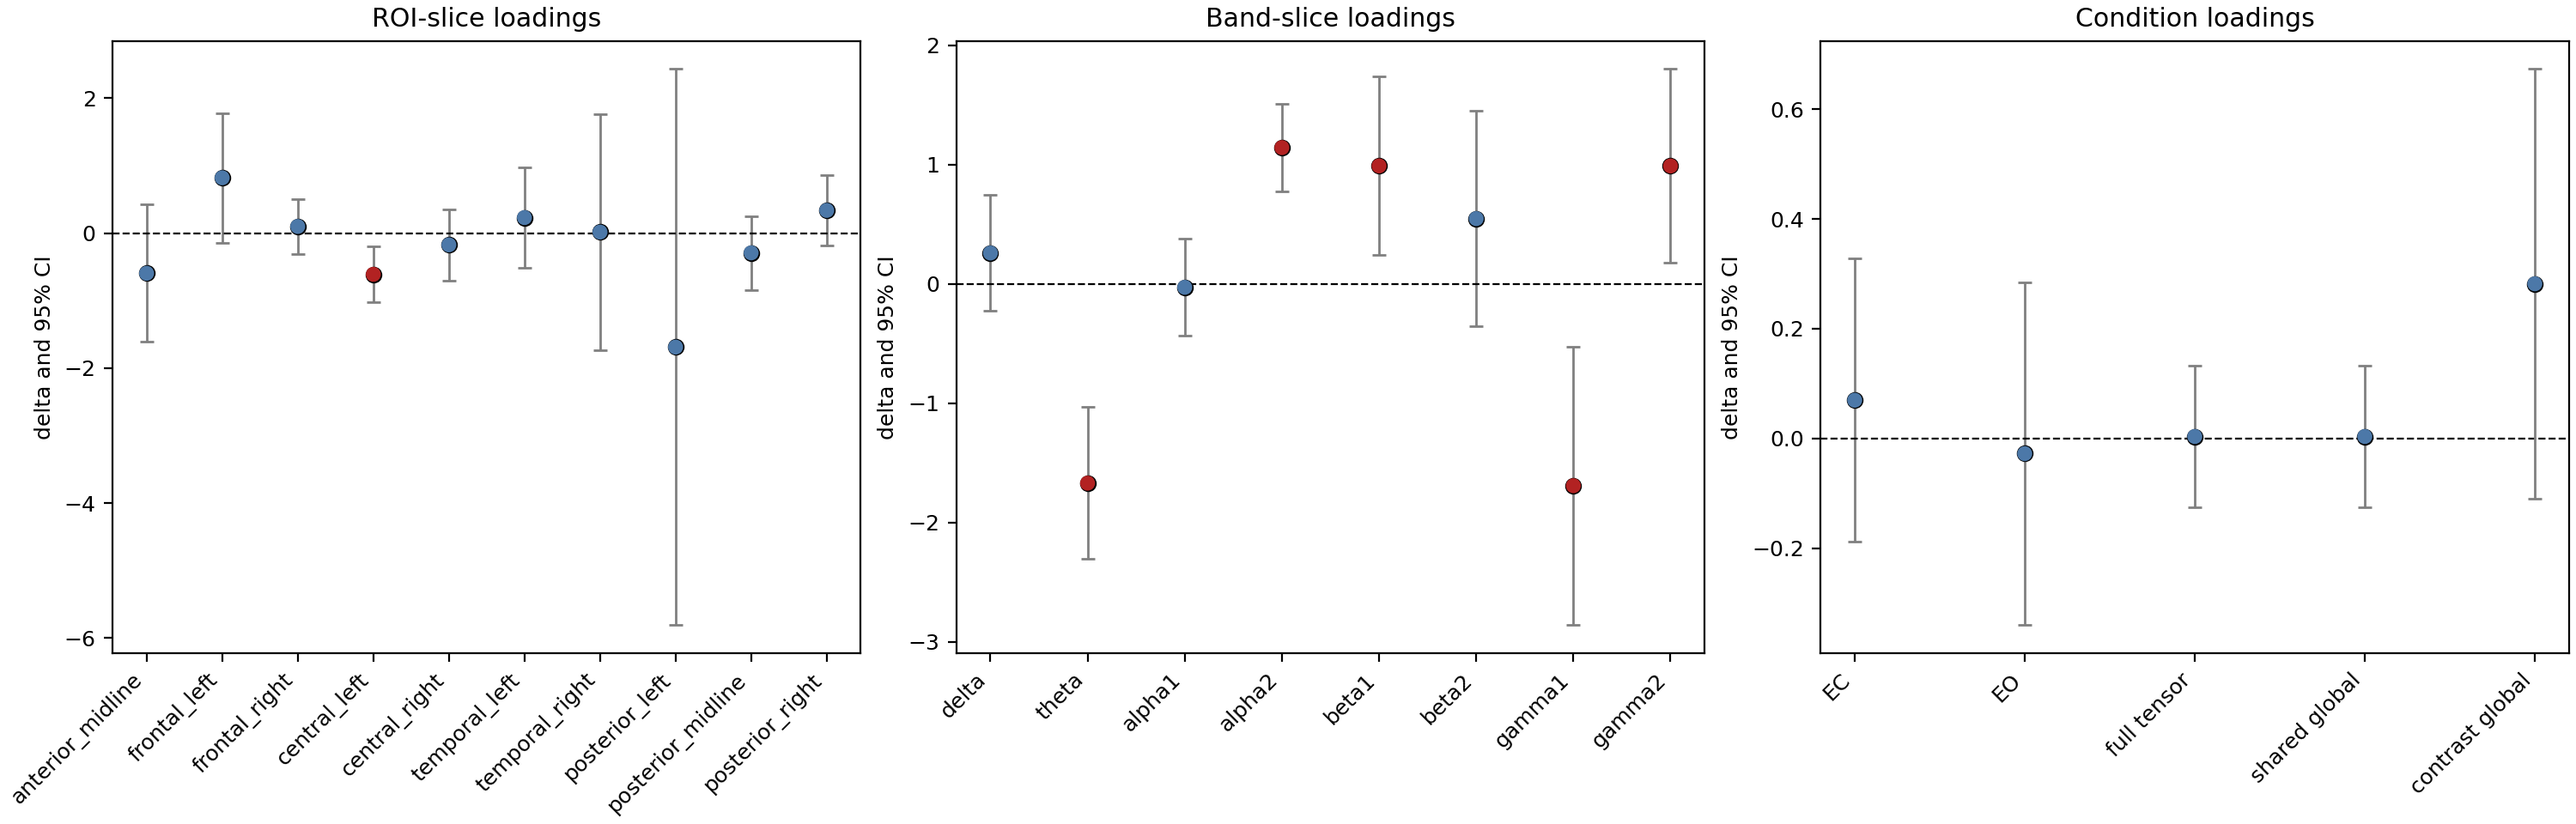
\includegraphics[width=\textwidth]{tsrproj_rank252_structured_loadings.png}
\caption{固定秩 $[2,5,2]$ 下的结构化 loadings：ROI-slice、band-slice 以及 condition/global summaries。红点表示对应 95\% 置信区间不包含 0。}
\label{fig:structured}
\end{figure}

\begin{figure}[H]
\centering
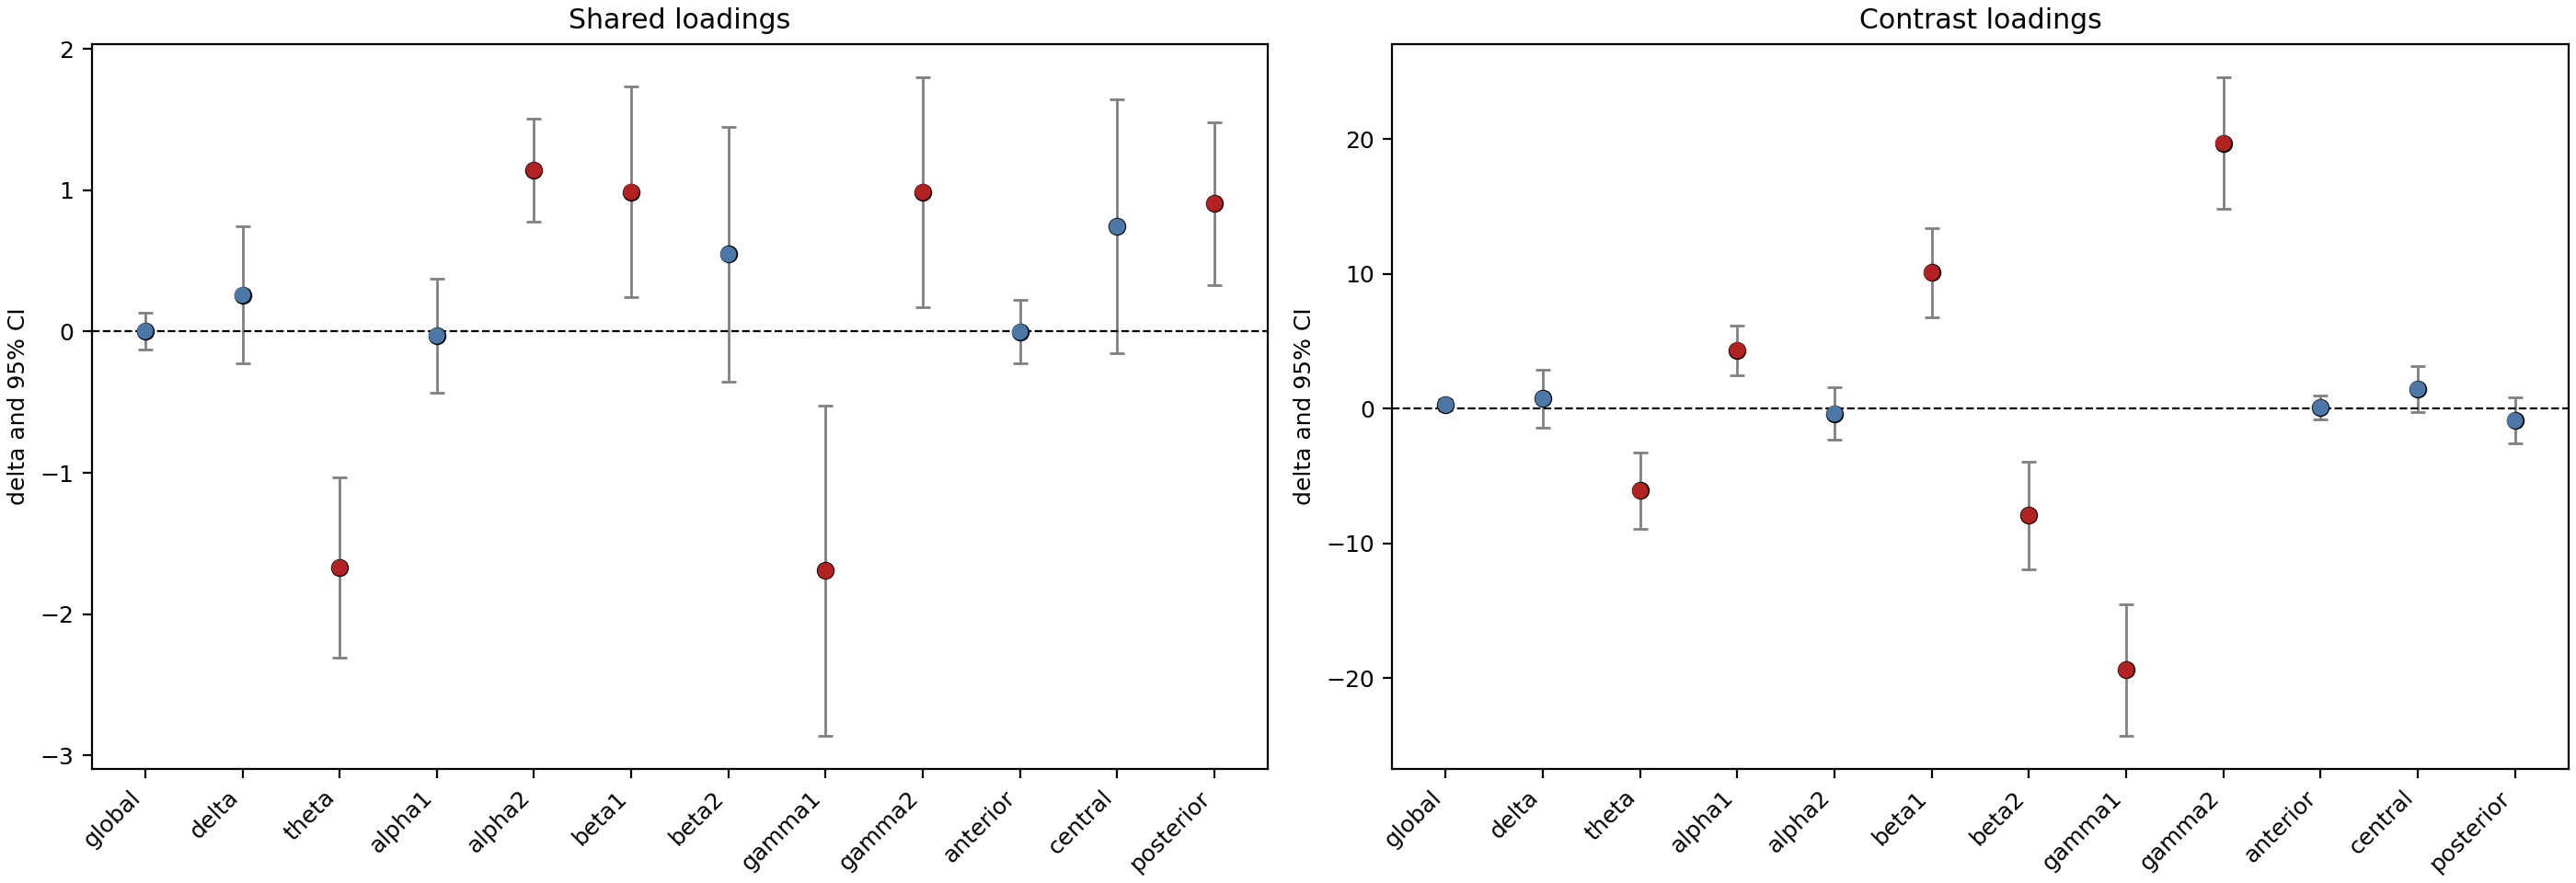
\includegraphics[width=\textwidth]{tsrproj_rank252_shared_contrast_loadings.png}
\caption{固定秩 $[2,5,2]$ 下的 shared 与 contrast loadings。红点表示对应 95\% 置信区间不包含 0。}
\label{fig:sharedcontrast}
\end{figure}

\section{结论}
在固定 Tucker 秩 $[2,5,2]$ 下，\texttt{tsrProj} 给出的统计推断结果表明：
\begin{enumerate}
\item 结构化显著性主要集中在 band-level summaries，而不是 global 或 condition-level averages；
\item ROI-level 的聚合证据较弱，仅 \texttt{central\_left} 与 \texttt{posterior} shared group 保持显著；
\item contrast-band 的信号明显强于 shared-global 或 contrast-global，说明 EC/EO 差异更多体现为特定频带方向上的结构，而不是整体平均偏移。
\end{enumerate}

从 sensitivity analysis 的角度看，固定秩 $[2,5,2]$ 的推断仍支持 ``频带结构强于整体平均结构'' 这一主结论，但相较于其他秩设定，空间层面的显著性更为保守。

\end{document}
